%%%%%%%%%%%%%%%%%%%%%%%%%%%%%%%%%%%%%%%%%%%%%%%%%%%%%%%%%%%%%%%%%%%
%                                                                 %
%                            CHAPTER FOUR                         %
%                                                                 %
%%%%%%%%%%%%%%%%%%%%%%%%%%%%%%%%%%%%%%%%%%%%%%%%%%%%%%%%%%%%%%%%%%%

\chapter{VERSIONING TABULAR DATA}\label{ch:spreadsheet}

The initial goal of the research sought to develop the method of calculating provenance distance between two data objects.
The value in this measure lies in determining whether similarity of the activities responsible for producing the objects provides context for reproducibility and result comparisons.
The "Noble gas isotopes in hydrocarbon gases, oils and related ground waters" database has the desirable qualities for this comparison of varied sizable provenance and multiple versions to provide comparable changes.
However, gaps appeared to hinder the approach with using provenance data to measure change distance.
To begin, each of the spreadsheet database's rows were considered to be a separate data object, as opposed to the individual file since this structure changes in the subsequent version, as explained later.
Each row contained an entry indicating the reference used to compile the readings stored, and this entry was used as the data entity to produce a provenance graph with the PROV model as seen in Figure \ref{CAM001ProvGraph}.
An important challenge to note when creating these graphs is that in version 1, the references were stored in a very human readable fashion.
The entry could be stored as a string or numeral even though all values were numbers.
In addition, the values were both comma separated and ranges indicated by a dash.
Version 2 of the database corrects many of these problems with consistent content type and presentation.
The documentation which accompanies the data set does not detail any changes to the compilation procedure that would indicate this improvement.
The conclusion then follows that even though the two data objects have essentially the same provenance graph, it does not capture the operational change which has occurred within the data.

\begin{figure}
	\centering
	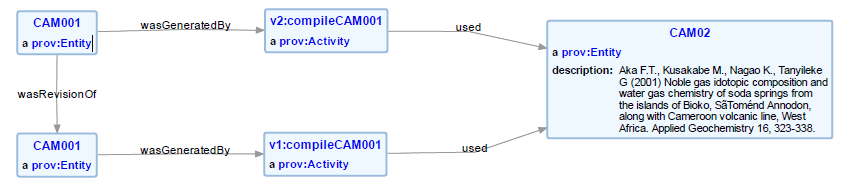
\includegraphics[scale=0.70]{figures/CAM001v1v2.png}
	\caption{Provenance graph for the entry CAM001 entry of the Noble Gas Database.  Other than the labels, the structure of each of the data objects is very much the same.}
	\label{CAM001ProvGraph}
\end{figure}

Version 2 also imposes many new changes that improve the data's readability.
This can be seen with the unification from files per region to a single file, reduction of columns, and better standardization of value format within a column.
The accompanying documentation includes instructions on how to read each column within the spreadsheet, but makes no mention as to the changes made to the original version to produce the current release.
In software, this would take the form of a change log, but they also provide the developer a chance to explain his or her motivation for making those changes.
In this case, an example would be the two versions reporting concentration in different units.
As a result, the first goal to quantify the amount of modification between the first and second versions needed a change log document to codify the differences. For small applications, a listing of modifications sufficiently explains the transition to a new data set, but for larger applications a machine-readable change log demonstrates potential for significant value as previously mentioned.

Lack of familiarity with the data set and it's authors immediately posed a challenge to verifying the resulting change log's validity.
The Paragenetic Mode for Copper Minerals database did not have these same constraints and also featured a more limited set of change.
With the process's validity now verifiable, the versioning model could now apply to the resulting change log, but at that point, the model still included capturing the actual values in the data object that changed.
Including the actual data into the change log gives concrete details as to how the object behaves when it changes, and is common practice.
However, when modeling the version, data within the object provides a level of granularity that does not transport well from one information system to the next.
In addition, the resulting linked data graph stores double the amount of data than the actual change, once for the linked data and again for the values.
As a result, the model leaves out including the data.
This allows the model to remain open and adapt to more complex versioning procedures.

The RDFa implementation in the HTML change log makes a trade-off that bends the original intent of the framework, but leverages its ability to translate into RDF.
RDFa natively adds context to describe specific text instances, such as a string of text being a name or another constituting a phone number, by encoding it in the format Subject Predicate Object.
The text being described appears as either the Subject or Object, and the remainder becomes implied from previous entries.
In the change log, no text string directly denotes a modification so it must be explicitly injected through the document source.
In addition, similar text entries appear close together, such as pairing column numbers with each other and keeping values side-by-side.
However, this does not follow the order in which objects appear to encode them into the model, meaning that relationships must often be explicitly defined.
The resulting source thus directly defines the entire relationship of the entries and objects into the graph without using any of the human readable parts of the log.
However, this means that RDFa parsers can directly extract the full linked data graph similar to the one in Figure \ref{CopperGraphVerGraph}.

\begin{figure}
	\centering
	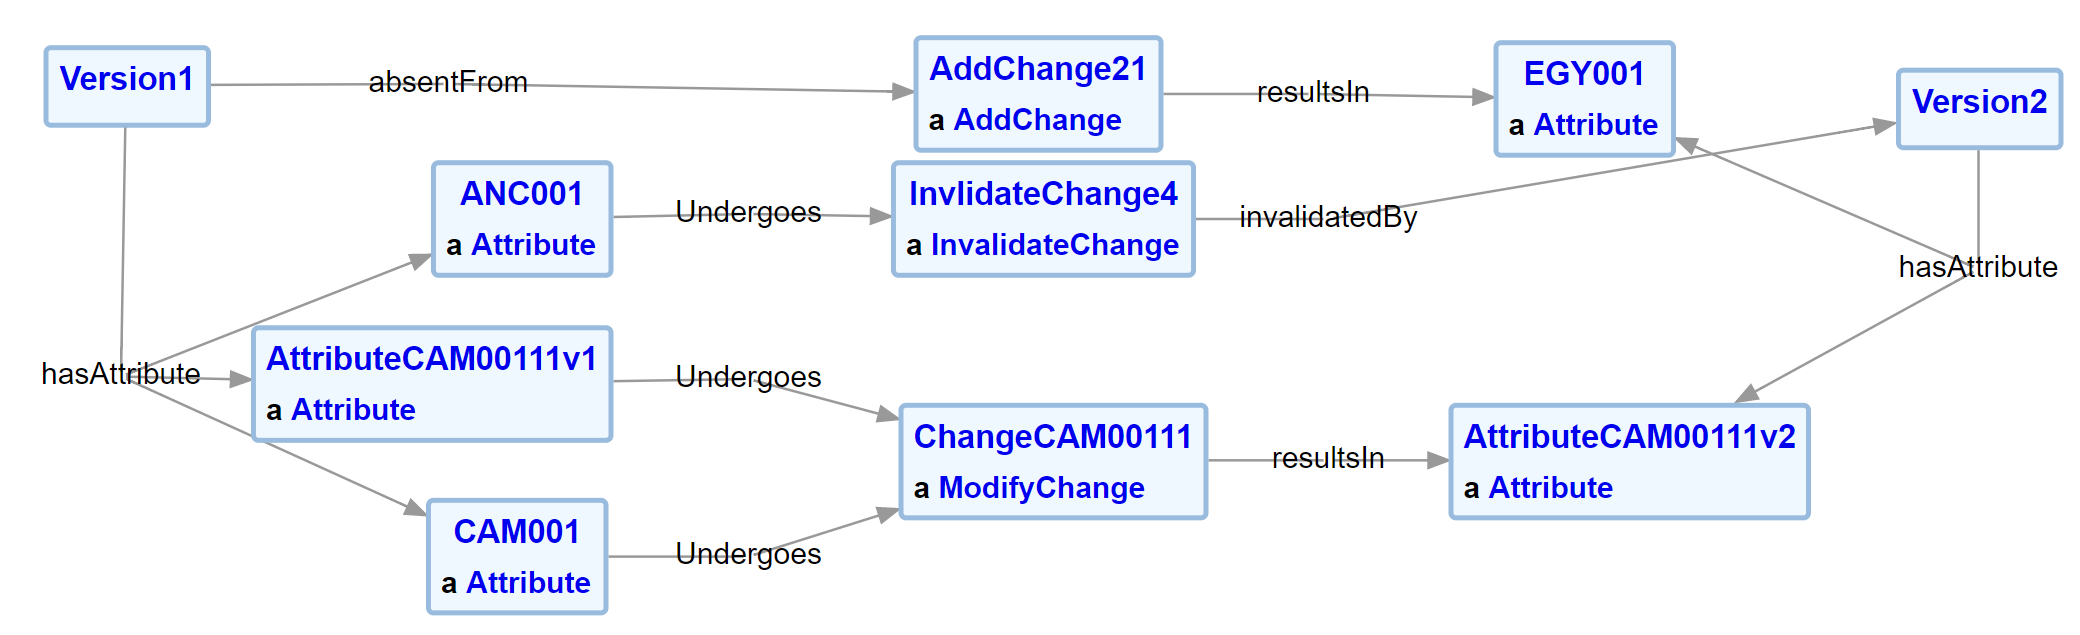
\includegraphics[scale=0.30]{figures/NobleVersion.png}
	\caption{Some initial entries from versions 1 and 2 of the Noble Gas dataset}
	\label{NobleGraph1}
\end{figure}

\begin{figure}
	\centering
	\begin{adjustbox}{addcode={\begin{minipage}{\width}}{
					\caption{Versioning Graph representing the linked data graph with selected entries of additions, invalidations, and modifications after the publication of the third version. 
			}\end{minipage}},rotate=90,center}
		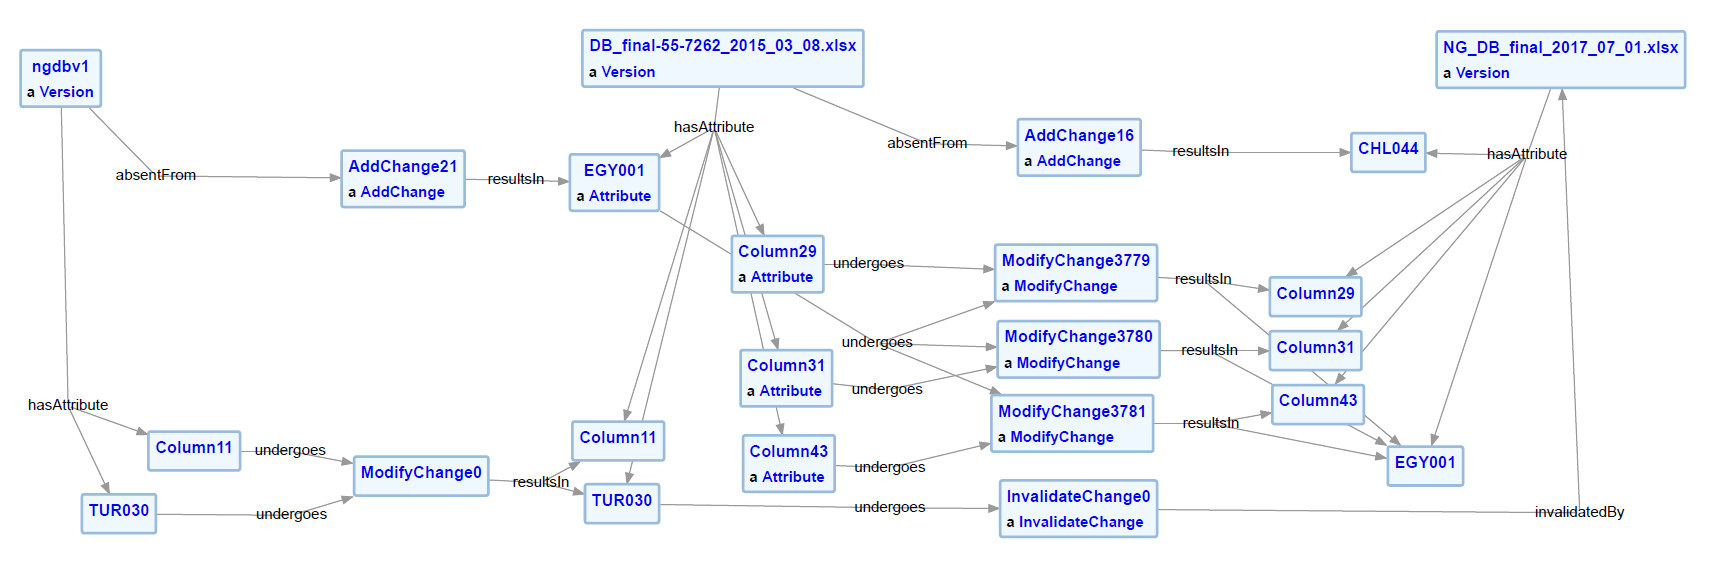
\includegraphics[scale=0.5]{figures/NobleVersion2.png}%
	\end{adjustbox}
	\label{NobleGraph2}
\end{figure}

\begin{figure}
	\centering
	\begin{adjustbox}{addcode={\begin{minipage}{\width}}{
					\caption{Versioning Graph representing the linked data graph with selected entries of additions, invalidations, and modifications. 
				}\end{minipage}},rotate=90,center}
		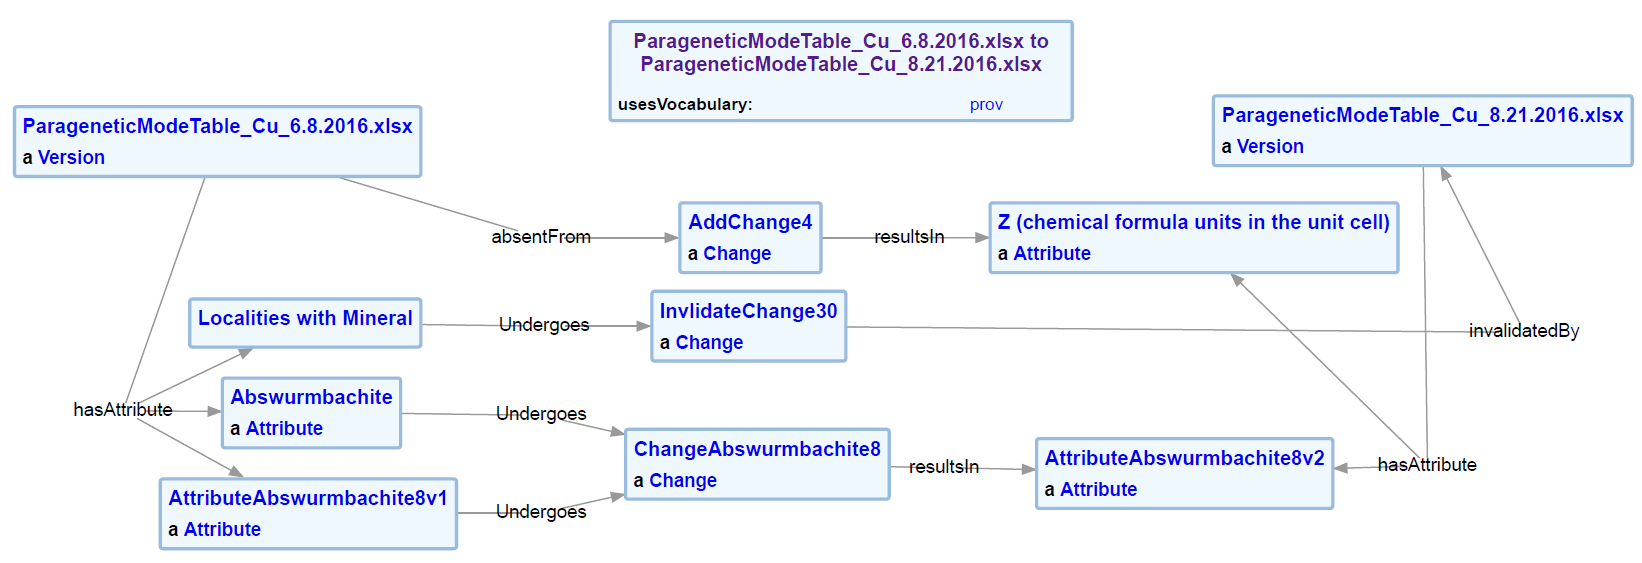
\includegraphics[scale=0.5]{figures/VersioningGraph2.png}%
	\end{adjustbox}
	\label{CopperGraphVerGraph}
\end{figure}